\documentclass{article}

% Language setting
% Replace `english' with e.g. `spanish' to change the document language
\usepackage[english]{babel}
%\usepackage{setspace}
%\doublespacing
% Set page size and margins
% Replace `letterpaper' with `a4paper' for UK/EU standard size
\usepackage[letterpaper,top=2cm,bottom=2cm,left=3cm,right=3cm,marginparwidth=1.75cm]{geometry}

% Useful packages
\usepackage{amsmath}
\usepackage{graphicx}
\usepackage[colorlinks=true, allcolors=blue]{hyperref}


\title{Twitter Natural Disaster Predictions with NLP}
\author{Tyusha Sarawagi & Sarah Wright}

\begin{document}
\maketitle
%https://www.overleaf.com/project/625ecd72b77aea4f91d90981

\begin{abstract}

Twitter can be a powerful tool, both as a resource for finding urgent information about situations around the globe and a tool for communicating useless information about sales and petty gossip. Hashtags are useful tools for shifting through the clutter, however, oftentimes they are misused, such as putting disaster terms like ``\#Hurricane" on a sale ad to increase views. This has made it difficult for professionals to identify important and relevant information in accordance with their needs. However, in the past decade, humans have become able to teach computers to examine the complex structure of the English language as the field of machine learning advances. This has become increasingly salient, as humans can no longer review  content created by social media because it is complex. The purpose of the research paper is to use a machine learning technique called  Natural Language Processing (NLP) to read through the tweets and  predict which tweets on Twitter are about natural disasters and which ones aren’t. Using a collection of Twitter disaster tweets, that calls for Natural Language Processing techniques, and pairing them with a Random Forest and Multinomial Naive Bayes Regressions, an accuracy of 80.6 percent was obtained. The findings are promising, and they could help the general population sort through and analyze information shared during times of mass crisis. 

\end{abstract}


\section{Introduction}

Social media has become a vital component of living in today's modern world. Because of the widespread use of smartphones and tablets, people can now announce and notify others in real-time of any emergency they are facing. Any crisis information shared on social media has the potential to save thousands of lives by informing others of emergencies and allowing them to take preventative action. Many agencies are attempting to examine tweets programmatically in order to detect natural disasters and emergencies \cite{6}. This type of effort can benefit millions of people who have access to the internet and can be notified in the event of an emergency or tragedy.

It is critical to collect vital and accurate information in order to respond to these disasters in a timely and efficient manner. The world saw during a pandemic that it is essential to respond quickly to people's requirements, which are conveyed in messages sent across multiple sources of media. In recent decades, social media platforms such as Twitter, Facebook, LinkedIn, and Instagram have proven to be essential hubs for information during natural and man-made disasters. However, it can also be seen that the accuracy, volume, and speed with which this data can be sorted through for any valuable information remain a key concern, particularly when it comes to a crisis. 

Machine learning algorithms such as natural language processing (NLP) could help categorize these messages so that they can be delivered to relevant disaster relief agencies that handle medical aid, water, shelter, food, logistics, and other services. This paper proposes an approach for predicting which tweets on Twitter are about natural disasters and which ones aren't. Because Twitter's data is in text form and has no modifications for a computer to easily understand in a numeric or short categorical form that can be used with a typical regression, Natural Language Processing (NLP) must be used to classify it into categories. The categories this paper uses are: ``related to disaster" = 1 and ``not linked to the disaster" = 0. On the test set constructed from the original data set, the paper makes a prediction and performs accuracy testing on the produced classifier model. 


\section{Data}
Twitter is a microblogging and social networking site based in the United States that allows users to share news, data, and thoughts. In an emergency or tragedy, and has become a crucial channel of communication. It also happens to be the source data used to assess the model. 

The model completed and referenced in this paper examines 7613 tweets, each with its twitter-id, location, a keyword chosen from the tweet, and a target indicating whether the tweet is mentioning a disaster or not. For example, using the keyword ``ablaze”, the model should be able to determine the difference between a tweet that says, ``#nowplaying Alfons – Ablaze 2015 on Puls Radio” having a target of 0 since it does not mention an actual disaster, and ``Birmingham Wholesale Market is ablaze BBC News – Fire breaks out at Birmingham's Wholesale Market" having a target of 1 since there is a disaster/emergency. 

Datasets that are not organized in a prescribed manner can be referred to as referred to as unstructured data. Unstructured data is usually textual, such as open-ended survey responses and social media discussions, but it may also be non-textual, such as photos, video, and audio. The data stored in Twitter's system is a set of unstructured data which is not in any specific format. This is where the actual difficulty in interpreting Twitter's data resides. Natural Language Processing (NLP) is necessary for this. After the data is pre-processed, the string tweets are then tokenized and subjected to analysis, which is further discussed in the Methods section.



\section{Exploratory Data Analysis (EDA)}
The dataset that is used to create and analyze tweets is  has no labeled author, but it is titled, ``Natural Language Processing with Disaster Tweets” and was posted by Kaggle.com \cite{9}. The data used, is divided into 2 datasets: a training set and a testing set. The training set consists of 7613 rows and five columns, and the testing set consists of 3263 rows and four columns (without the target column). Here are some of our findings from the dataset without the model. 

In the bar chart labeled, Distribution of Target Counts (Figure 1), it can be seen that there is an imbalance in the data provided. There are more non-disastrous tweets included in the dataset than there are disastrous, which can be expected. This information may influence the final classifier being developed. For example, the classifier may have more bias toward predicting the dominant class, which in our case is non-disastrous tweets. 

\begin{figure}[!h]
    \centering
    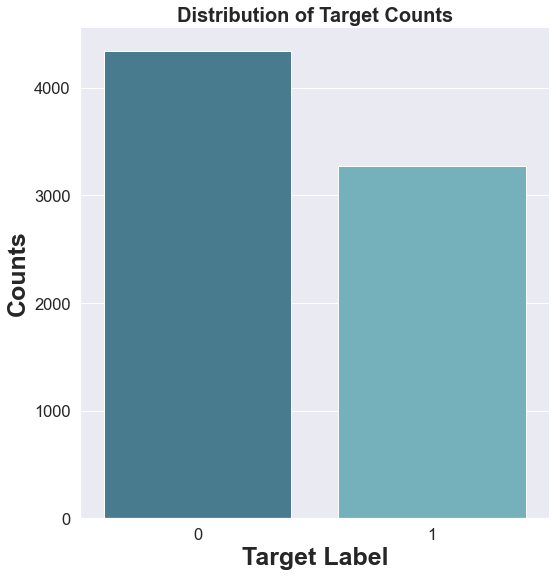
\includegraphics[width=0.55\textwidth, left]{bar.png}
    \caption{Histogram of Target Distribution}
    \label{fig:bar}
\end{figure}

Visualizing texts on typical plots like bar plots, line plots, or scatter plots can be challenging when dealing with NLP data. Instead, to visualize common words in our dataset, a word cloud can be used. In the word cloud above (Figure 2) is the word cloud that represent the data from the entire dataset. The terms that appear in the biggest are the ones that appear in the dataset the most frequently. Figure 2 shows us that the words ``emergency”, ``disaster”, ``fire”, ``storm”, ``suicide”, ``burning” occurred more frequently in the text data as compared to others. 

In the two clouds below, Figure 2(a) and  Figure 2(b) shows a comparison between the elements with a target 1 or 0. Figure 2(a) represents the word cloud drawn from the non-disastrous tweets (only). From this information, it can be seen that the word that is most frequently used are ``body” and ``emergency”. The word ``body” does not happen to, not be a disastrous word, however ``emergency” is a word that can create some confusion, especially when compared to Figure 2(b). Other words seen in the word cloud depict an equal frequency of words, since most of the words appear in the same size.

Figure 2(b) represents the word cloud drawn from the disastrous tweets (only) and once again the words that have a bigger text are more frequently used and are also disaster related words. For instance, ``suicide”, ``emergency”. ``bombing”, ``storm”, “fire” are the words whose size is bigger compared to other words in the cloud. Furthermore, there are a lot more words that are in bigger size, which means they are used frequently in contrast to figure 2(a). However, there is some overlap such as with the word ``emergency”. 

\begin{figure}[!h]
    \centering
    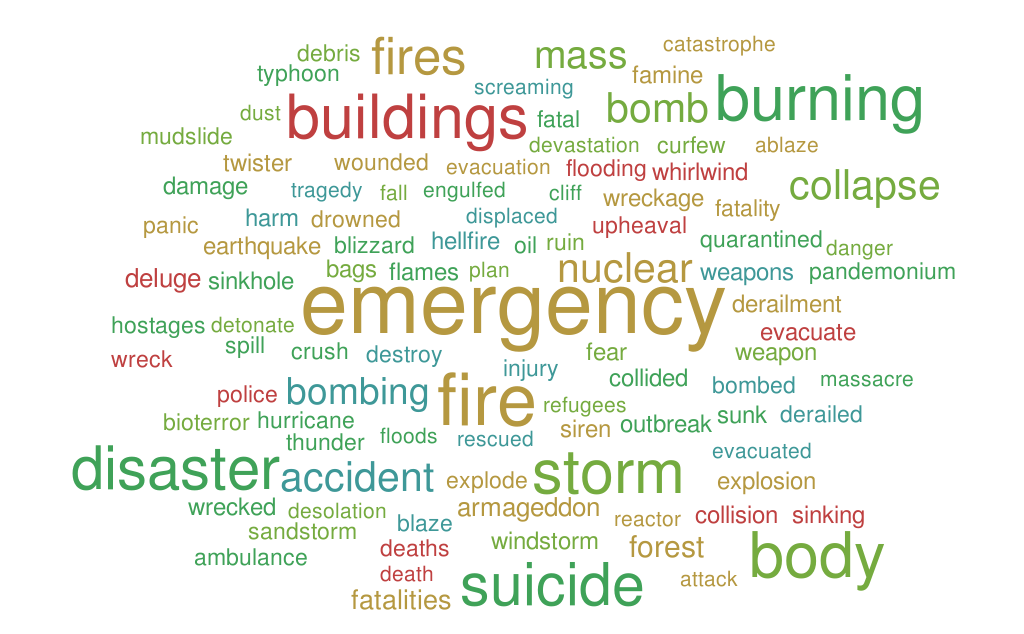
\includegraphics[width=0.7\textwidth, left]{wordcloud.png}
    \caption{Wordcloud of all the keywords}
    \label{fig:wordcloud}
\end{figure}


\begin{figure}
\centering
\begin{minipage}{.5\textwidth}
  \centering
  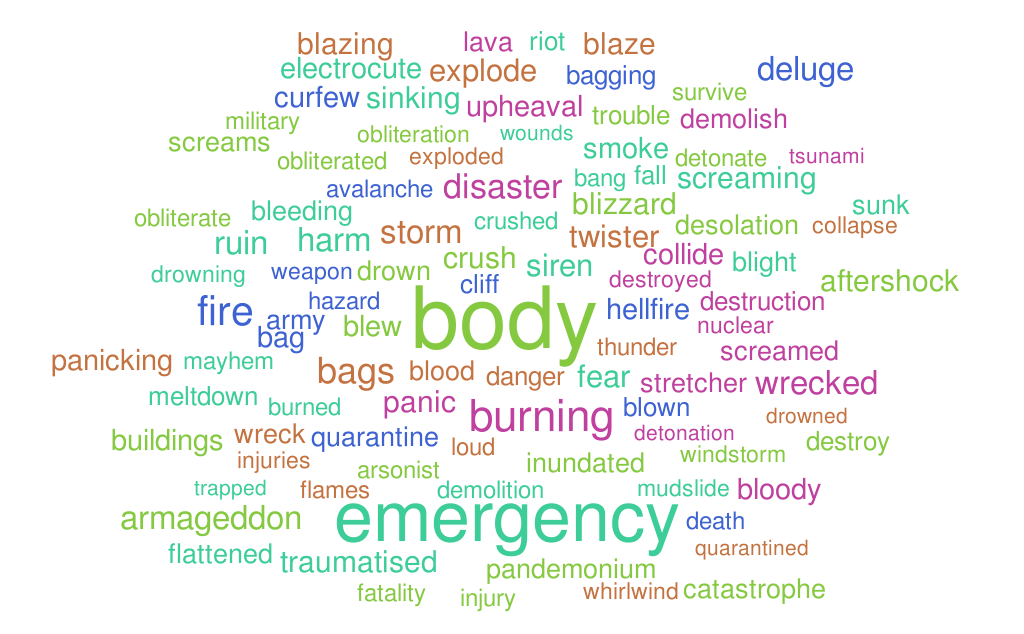
\includegraphics[width=1.2\linewidth]{0wordcloud}
  \captionof{(a)}{ Wordcloud for non-disastrous tweets}
  \label{fig:0wordcloud}
\end{minipage}%
\begin{minipage}{.5\textwidth}
  \centering
  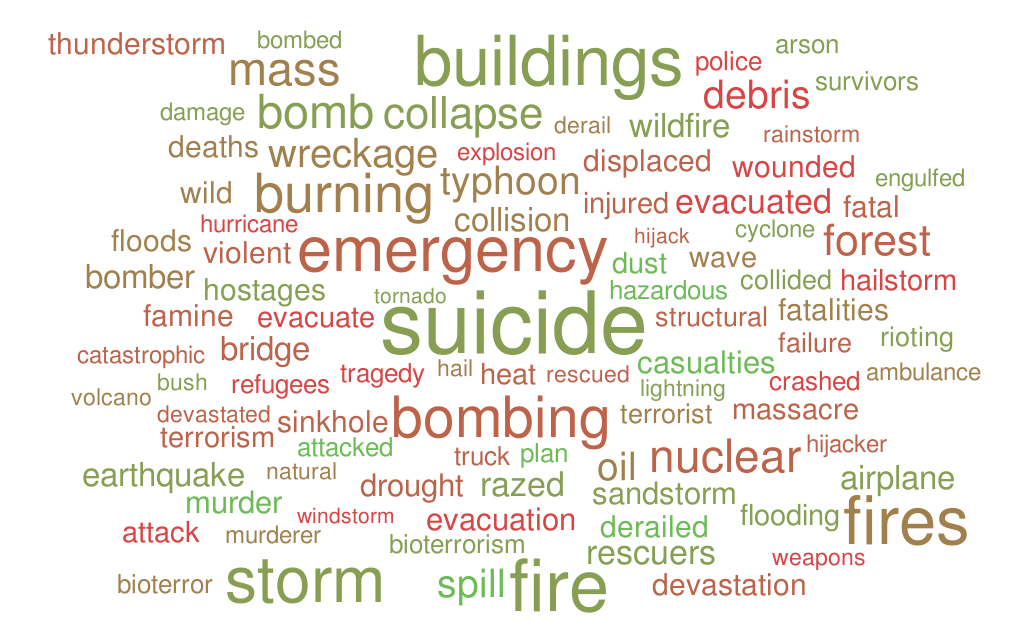
\includegraphics[width=1.2\linewidth]{1wordcloud}
  \captionof{(b)}{ Wordcloud for disastrous tweets}
  \label{fig:1wordcloud}
\end{minipage}
\end{figure}
\pagebreak

Within the dataset there are, 4521 unique locations. To see where most of the data was located, Figure 3 shows the top ten countries from the dataset since it would be almost impossible to plot all the locations. Many of these locations are unusable, such as ``Anime World” and ``Yeezy Taught Me, ``NV”. Additionally, the cities that appeared in the top ten locations are listed with corresponding countries in the Map shown in Figure 3 labeled ``Tweet Locations of Top 10 Countries”. It's possible that some cities remain in the remainder of the dataset, which is something to think about in the final model.


\begin{figure}[!h]
    \centering
    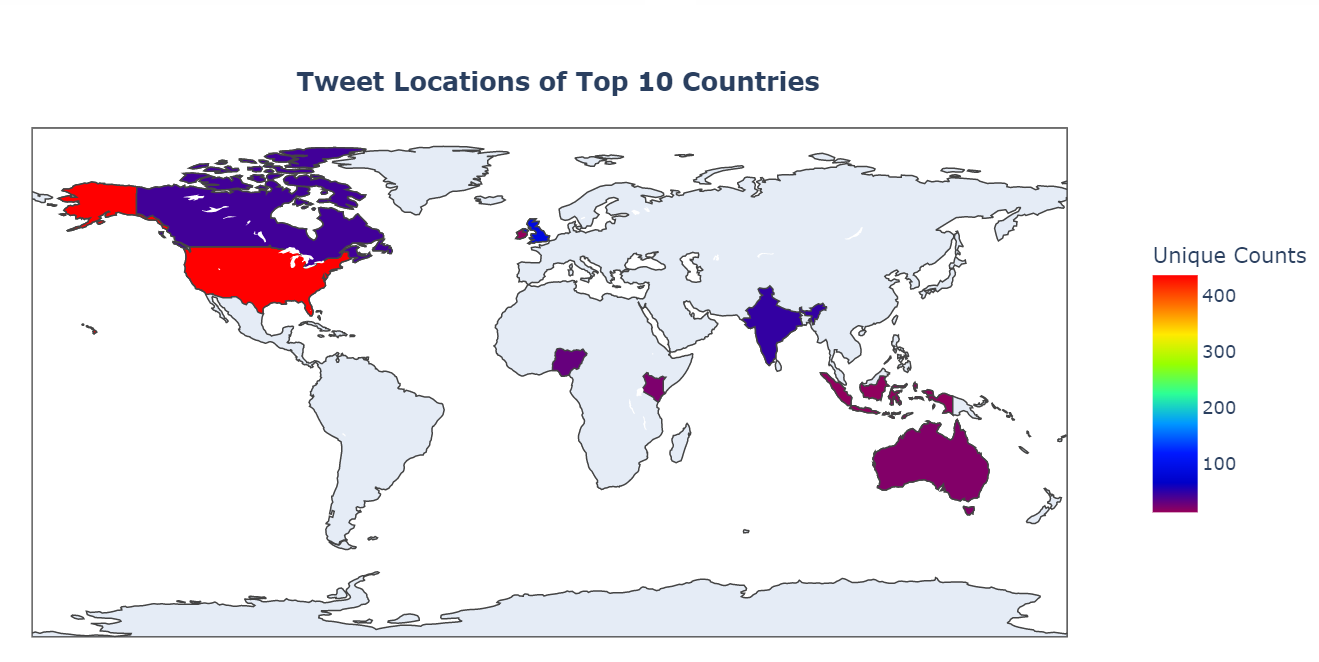
\includegraphics[width= 0.9\textwidth, left]{map.png}
    \caption{Heatmap of Tweets from Top 10 Countries}
    \label{fig:map}
\end{figure}

\section{Methods}
\subsection{Pre-Processing}

The goal of the research paper is to predict whether each tweet is describing a natural disaster or not, using a collection of Twitter disaster tweets tagged with the essential keywords, the location of the tweet, and the comment/tweet itself. The aim is to make a prediction based on the meaning of the word and ability to classify them into significant or insignificant. 


The data being used (including the results) are completely categorical, and to conduct sentimental analysis, a different method of prediction needs to be used.  For this project, Natural Language processing (NLP) is the intended method, which is an unsupervised learning method used to conduct research. Natural language processing (NLP) refers to the branch of computer science that helps computers communicate with humans in their own language and scales other language-related tasks. NLP allows computers to read text, hear voice, analyze it, gauge sentiment, and identify which bits are significant. Machines can now interpret more language-based data than humans can, without becoming fatigued and in a consistent and fair manner. Given the massive volume of unstructured data created every day, from medical records to social media, automation will be essential for efficiently analyzing text and audio data. The goal of this research is to use NLP to read through the tweets and the other predictors (tweet text, location, keywords) and determine whether there is a Natural Disaster or Not in the location specified. 


\subsection{Text & Speech Processing}
Text and speech processing allows the computer to understand the text that is being read into the system. There are several types of Processing methods like Tokenization, Keyword Extraction, Text Classification and many more. Some of the methods use while analyzing the model in this paper are discussed below. 

\subsubsection{Tokenization}

Tokenization is a method of segmenting a string of words into meaningful components that can be analyzed. In simple terms, it is the process of breaking down a phrase, sentence, paragraph, or even an entire text document into smaller components like individual words or phrases. Each of these smaller units are called tokens. This process allows to read in the data in the dataset as strings of text and then split them up so that it can be analyzed and the values could be attached to each segmented part of the string pulled in. From there, the frequency of each word and whether it is a good predictor of natural disasters can be tested.


%To do this, we will run the following python libraries: . This will prevent x and automatically do y. 

\subsubsection{Stop Word Removal}

Stop word removal is one of the most used preprocessing processes in many NLP applications. In any language, there are plenty of stop words. Stop words are the words in natural language that have very little meaning, such as ``is", ``are", ``an", and ``the", etc. By deleting these words, low-level information from our text can be eliminated, allowing us to focus more on the crucial information. Furthermore, because there are fewer tokens involved in the training, removing stop words reduces the size of the dataset and thus reduces training time. Also, removing such phrases has no adverse impact on the meaning of the sentence while being analyzed by the computer and it helps the model.


\subsubsection{Lemmatization}
Lemmatization is the process of grouping words that have similar meaning based on a dictionary into their normalized form \cite{3}. This process of Lemmatization overlaps with stemming. It makes the work so much easier because it uses dictionary definitions to group similar words together. Using Lemmatization words like ``saw" and ``see" could be grouped together while with stemming, the grouping would just be `s' \cite{4}.



%Before conducting this process, we looked at several research articles and the one I would like to mention is this one and their process. \cite{NLP}


\subsection{Morphological Analysis}
Morphological analysis is the process of making the tokenized and lemmatized strings usable. During this process, any words or characters that are not of consequence are removed from the text. Morphological analysis of a word offers information such as number, gender, and so on. This information can be utilized to produce the right form of the word in the target language. This is a multi step process that is similar to Data Cleaning. Some methods of morphological analysis used in research paper are discussed below.

\subsubsection{Bag-of-Words/ Count Vectorization}
The bag-of-words (BOW) model is a representation that counts how many times each word appears in any text to generate fixed-length vectors. In bag-of-words technique the frequency of each word is used as a feature for training a classifier. This process is often called as vectorization. As the name may suggest, the bag-of-words technique does not consider the position of a word in a document. A limitation of bag-of-words technique is that it does not bring in any information on the meaning of the text. For example, considering these two sentences, ``Studying is easy but tedious” and ``Studying is tedious but easy”, a bag-of-words model would create the same vectors for both of them even though they have different meanings.


\subsubsection{Term Frequency Inverse Document Frequency (TFIDF)}

TFIDF (term frequency-inverse document frequency) is a statistical measure that evaluates how relevant a word is to a document in a collection of documents. This is done by multiplying two metrics: how many times a word appears in a document, and the inverse document frequency of the word across a set of documents \cite{10}. TFIDF works by proportionally increasing the number of times a word appears in the document but is counterbalanced by the number of documents in which it is present. Hence, words like `this’,   `are’ etc., that are commonly present in all the documents are not given a very high rank. However, a word that is present too many times in a few of the documents will be given a higher rank as it might be indicative of the context of the document \cite{11}.

Term Frequency: It is defined as the number of times a word (i) appears in a document (j) divided by the total number of words in the document \cite{11}.

\[t f_i,j = \frac{n_i,j}{\sum n_i,j}\]
     

Inverse Document Frequency: It refers to the log of the total number of documents divided by the number of documents that contain the word. The logarithm is added to dampen the importance of a very high value of IDF \cite{11}.

\[idf(w) = log(\frac{N}{df_t})\]
      

TFIDF is computed by multiplying the term frequency with the inverse document frequency \cite{11}.

\[w_i,j = {tf_i,j} * log(\frac{N}{df_t})\]



\subsubsection{Part-of-Speech Tagging}

Part-of-Speech Tagging is the process of grouping words in a text in relation with a particular part of speech, based on the definition of the word and its context. Because certain words might represent more than one part of speech at various times and because some parts of speech are complicated. Part-of-Speech tagging is more difficult than just having a list of words and their parts of speech. The tag in case of is a part-of-speech tag signifies whether the word is a noun, adjective, verb, and so on. It can also be used to identify examples of grammatical or linguistic patterns without using a specific word, such as finding examples of any plural noun that isn't preceded by an article.



\section{Modeling}

\subsection{Sentimental Analysis}
The next step of the research is to use Sentimental Analysis on the Tokenized and preprocessed strings of text. Sentimental Analysis is the part of the process where words are used in context to make our prediction. There are a few methods that can be used: a Machine Learning Method, a Lexicon Method, or a Hybrid of the two methods \cite{1}. The methods of modeling used for this research are supervised learning methods: Random Forest Classifier and Naive Bayes model.

\begin{figure}[!h]
    \centering
    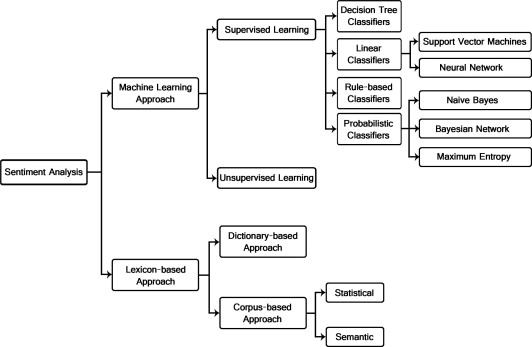
\includegraphics[width=0.7\textwidth, left]
    {Supervised_Learning_Methods.jpg}
    \caption{Methods of Sentimental Analysis}
    \cite{5}
    \label{fig:SentimentalAnalysis}
\end{figure}


\subsubsection{Random Forest Classifier}
Random forest is a supervised machine learning algorithm that is commonly used to solve classification and regression issues. It is called random forest because  the subsets of the variables are random, and forest because there are lots of decision trees, which is another  method of Machine Learning. By training the trees on different subsets of the factors, the resulting trees decorrelate and prevent single factors from dominating. One of the most essential characteristics of the Random Forest Algorithm is that it can handle data sets with both continuous and categorical variables, as in regression and classification. Random Forest creates decision trees from several samples, using the majority vote for classification and the average for regression. The number of decision trees used for the model in the paper is 300. It can be changed according to the kind of accuracy required for the model,  however there are trade-offs. 



\subsubsection{Naive Bayes Model}

Naive Bayes classifiers are a type of basic ``probabilistic classifiers" based on Bayes' theorem and strong independence assumptions between features in machine learning. All Naive Bayes classifiers assume that the value of one feature is independent of the value of any other feature. Bayes' theorem is used in Naive Bayes classifier algorithms. The basic insight of Bayes' theorem is that when new data is provided, the probability of an event may be changed. The Naive Bayes method in this model looks at specific keywords in a review to determine whether it is favorable or negative, based on the output set. Naive Bayes Classifier has three different algorithms: Guassian naive bayes, multinomial naive bayes, bernoulli naive bayes. For the modeling done for the research paper, multinomial naive bayes model is being used. Multinomial naive bayes is commonly used in multinomial event models such as bag-of-words, which is a way of representing a document as vector space by counting words.


\section{Results}

Two models were created for predicting and sorting tweets into two categories: those that belong to disaster-related tweets and those that don't. First is the Random Forest method and second is the Multinomial Naive Bayes Model. Initially when running these two models, the accuracy was at 75 percent, however after adding the additional steps of Lemmatization and Part of Speech Tagging into the preprocessing methods the accuracy average between the two methods increased by 5.6 percent. From these two models, the average accuracy percentage obtained was  about 79.7 percent. The random forest model had an accuracy of about 78.915 percent and the accuracy of the Multinomial Naive Bayes was about 80.604 percent, as presented in the figure below (Figure 5). Overall, there was not much of a difference in the accuracy of the models when parameter tuning when cross validation was applied. The parameter tuned Multinomial Naive Bayes model only achieved a slightly higher accuracy. This is due to the fact that every variable in the model are independent of each other. 


\begin{figure}[!h]
    \centering
    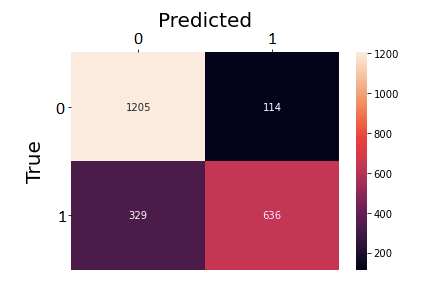
\includegraphics[width=0.607\textwidth, left]{heatmap.png}
    \caption{Heatmap of the Confusion Matrix}
    \label{fig:bar}
\end{figure}


\section{Discussion}

Globally, disasters and crises occur on a regular basis. People can now convey the occurrences of disasters they are experiencing in real-time, thanks to the popularity of cellphones, laptops, and tablets. News organizations and disaster relief organizations are attempting to monitor tweets in real-time in order to detect calamities \cite{6}. Millions of ordinary people would benefit from this, as it would help them avoid potential disasters. People could take preventative action if they were notified in real-time about the occurrence of disasters in a specific place. The outcomes of this article indicate that twitter data can be appropriately sorted into categories with a good degree of accuracy.

This paper proposes an approach for predicting which tweets on Twitter are about natural disasters and which ones aren't. There are 222 unique keywords in the dataset. Some of them have the same meaning but in various forms (e.g. dead and death, weapon and weapons, etc). Some keywords can be merged to minimize the number of distinct keywords to increase accuracy and optimize the model. Various preprocessing techniques were used in the research paper, but there are many areas in which these models can be improved upon to obtain a better accuracy at classifying tweets. For instance, some advanced techniques like feature extraction, stemming, machine translation, text classification, urgency detection, speech recognition and so on. Due to lack of time and experience, these techniques are not used in this paper. A simplified and more clear text can help us build a more informative model, resulting in a better accuracy and performance. 

Finally, performing the models on the bigrams and trigrams that would result in a significant improvement of the model. This would provide the algorithm a better understanding of how the terms in the tweet are employed. Because the research only considered unigrams, it's extremely possible that adding bigrams and trigrams as data features will improve accuracy.


%\cite{introduction}: what is sentimental analysis. 
%add a comparison between word clouds 
%add more data viz about making our assumption as to what words will be the best predictors of success 
%3rd person 
% space then cite then period. 
%equations 
%4.2 2nd par what did we pick?
%CONSISTENT CItations : ref 2, ref 1
%what 














%\cite{1, 2, 3, 4,5,6,7,8}
\pagebreak
\bibliographystyle{ieeetr}
\bibliography{sample.bib}
\end{document}














